\documentclass[conference]{IEEEtran}
\IEEEoverridecommandlockouts
\usepackage{cite}
\usepackage{amsmath,amssymb,amsfonts}
\usepackage{algorithm}
\usepackage{algorithmic}
\usepackage{graphicx}
\usepackage{textcomp}
\usepackage{xcolor}
\usepackage{booktabs}
\usepackage{array}
\usepackage{url}
\usepackage{tikz}
\usetikzlibrary{arrows.meta,positioning,calc,fit,backgrounds,shapes.geometric}
\graphicspath{{./}{figures/}}
% Every reported result is a macro generated by proran.care_report.
% Results generated by proran.care_report from the saved per-seed runs.
% Do not edit by hand; regenerate with scripts/build_submission.py.
\newcommand{\NoResHSR}{51.6}
\newcommand{\NoResOutage}{5.42}
\newcommand{\NoResFull}{75.3}
\newcommand{\ReactiveQoS}{66.2}
\newcommand{\ReactiveURLLCQoS}{65.4}
\newcommand{\CertaintyHSR}{83.1}
\newcommand{\CertaintyFull}{66.3}
\newcommand{\CertaintyDisplaced}{7.47}
\newcommand{\CertaintyUtility}{-0.18}
\newcommand{\FloorJITUtility}{12.56}
\newcommand{\FloorJITLead}{7.30}
\newcommand{\TunedUtility}{12.59}
\newcommand{\SliceTunedUtility}{12.65}
\newcommand{\CareHSR}{87.4}
\newcommand{\CareQoS}{51.7}
\newcommand{\CareOutage}{1.42}
\newcommand{\CareDisplaced}{0.92}
\newcommand{\CareURLLCQoS}{50.9}
\newcommand{\CareUtility}{12.38}
\newcommand{\CareLead}{5.22}
\newcommand{\VsReactiveUtilDiff}{+1.67}
\newcommand{\VsReactiveUtilLow}{+1.31}
\newcommand{\VsReactiveUtilHigh}{+2.03}
\newcommand{\VsReactiveUtilP}{0.00022}
\newcommand{\VsReactiveHSRDiff}{+3.91}
\newcommand{\VsFixedUtilDiff}{+1.64}
\newcommand{\VsFixedUtilP}{0.00022}
\newcommand{\VsFloorJITUtilDiff}{-0.18}
\newcommand{\VsFloorJITUtilLow}{-0.29}
\newcommand{\VsFloorJITUtilHigh}{-0.07}
\newcommand{\VsFloorJITUtilP}{0.0741}
\newcommand{\VsTunedUtilDiff}{-0.21}
\newcommand{\VsTunedUtilLow}{-0.34}
\newcommand{\VsTunedUtilHigh}{-0.08}
\newcommand{\VsTunedUtilP}{0.0705}
\newcommand{\VsSliceTunedUtilDiff}{-0.27}
\newcommand{\VsSliceTunedUtilLow}{-0.43}
\newcommand{\VsSliceTunedUtilHigh}{-0.11}
\newcommand{\VsSliceTunedUtilP}{0.0529}
\newcommand{\VsSliceTunedFullDiff}{-0.09}
\newcommand{\VsSliceTunedFullP}{0.00169}
\newcommand{\VsCareUncalUtilDiff}{+0.23}
\newcommand{\VsCareUncalUtilP}{0.0483}
\newcommand{\VsCareUncalHSRDiff}{+3.22}
\newcommand{\VsCareUncalHSRLow}{+2.39}
\newcommand{\VsCareUncalHSRHigh}{+4.04}
\newcommand{\VsCareUncalHSRP}{0.00022}
\newcommand{\VsCareUncalHSRWins}{19}
\newcommand{\VsCareUncalOutageDiff}{-0.37}
\newcommand{\VsCareUncalOutageP}{0.00022}
\newcommand{\FrontQuarterTunedDiff}{-0.59}
\newcommand{\FrontOneTunedDiff}{-0.21}
\newcommand{\FrontOneCareSingleDiff}{-0.02}
\newcommand{\FrontFourTunedDiff}{-0.05}
\newcommand{\FrontFourCareSingleDiff}{+0.79}
\newcommand{\FrontFourCareSingleP}{0.00117}
\newcommand{\FrontFourCarePPODiff}{+6.45}
\newcommand{\FrontFourCarePPOP}{0.00011}
\newcommand{\FrontSixteenTunedDiff}{-0.25}
\newcommand{\FrontSixteenTunedP}{0.00824}
\newcommand{\FrontSixteenCareSingleDiff}{+3.86}
\newcommand{\FrontSixteenCareSingleP}{0.00011}
\newcommand{\FrontSixteenCarePPOOnPolicyDiff}{+18.48}
\newcommand{\AblFullHSR}{87.8}
\newcommand{\AblNoRetimeHSR}{78.8}
\newcommand{\AblFreeActHSR}{60.6}
\newcommand{\AblFreeActReject}{48.9}
\newcommand{\AblSingleHSR}{85.0}
\newcommand{\LegacyNoResHSR}{51.6}
\newcommand{\LegacyFixedHSR}{59.6}
\newcommand{\CalBrier}{0.044}
\newcommand{\CalECE}{0.013}
\newcommand{\CalAUC}{0.897}
\newcommand{\ConstBrier}{0.083}
\newcommand{\ConstECE}{0.170}
\newcommand{\CalBaseRate}{94.2}
\newcommand{\CalFitExamples}{41{,}648}
\newcommand{\CalTestExamples}{42{,}661}
\newcommand{\CalAccLeadOne}{99.8}
\newcommand{\CalAccLeadEight}{70.1}
\newcommand{\ForecastPosRMSE}{2.59}
\newcommand{\ForecastDemandMAE}{1.66}
\newcommand{\ForecastScore}{0.77}
\newcommand{\ForecastTrainExamples}{175{,}104}
\newcommand{\TunedRuleQuarter}{floor/now, $\tau=0.0$}
\newcommand{\TunedRule}{floor/jit, $\tau=0.9$}
\newcommand{\LamQuarterFloorJITUtil}{14.12}
\newcommand{\LamQuarterTunedUtil}{14.70}
\newcommand{\LamQuarterTunedDisplaced}{5.62}
\newcommand{\LamQuarterTunedContracts}{437.9}
\newcommand{\LamQuarterCareUtil}{14.10}
\newcommand{\LamQuarterCareHold}{23.7}
\newcommand{\LamQuarterCareDisplaced}{1.15}
\newcommand{\LamQuarterCareContracts}{275.4}
\newcommand{\LamSixteenFloorJITUtil}{-18.73}
\newcommand{\LamSixteenCareHold}{2.0}
\newcommand{\CareWaitEMBB}{64.8}
\newcommand{\CareFloorEMBB}{33.5}
\newcommand{\CareWaitURLLC}{71.6}
\newcommand{\CareFloorURLLC}{23.4}
\newcommand{\CareDemandURLLC}{3.6}
\newcommand{\CareUpperURLLC}{1.4}
\newcommand{\CareWaitMMTC}{82.4}
\newcommand{\CareFloorMMTC}{17.5}
\newcommand{\SwUesFortyEightNoResHSR}{22.3}
\newcommand{\SwPrepThreeTunedHSR}{85.8}
\newcommand{\SwPrepThreeCareHSR}{79.4}
\newtheorem{proposition}{Proposition}
\renewcommand{\topfraction}{0.9}
\renewcommand{\dbltopfraction}{0.9}
\renewcommand{\textfraction}{0.1}
\renewcommand{\floatpagefraction}{0.8}
\renewcommand{\dblfloatpagefraction}{0.8}
\setcounter{topnumber}{3}
\setcounter{dbltopnumber}{2}
% Print a generated signed difference such as +3.22 without its sign.
\def\nosignaux#1#2\relax{\ifx+#1#2\else#1#2\fi}
\newcommand{\nosign}[1]{\expandafter\nosignaux#1\relax}
\renewcommand{\algorithmicrequire}{\textbf{Input:}}
\renewcommand{\algorithmicensure}{\textbf{Output:}}
\def\BibTeX{{\rm B\kern-.05em{\sc i\kern-.025em b}\kern-.08em
    T\kern-.1667em\lower.7ex\hbox{E}\kern-.125emX}}

\begin{document}

\title{CARE: Calibrated, Counterfactually Attributed Proactive Resource Reservation for Network-Sliced 5G Handovers}

% All authors share one affiliation: edit the department and institution here.
\author{\IEEEauthorblockN{Mayur Raju (24BCS073), Naramsetti Charan Raj Gupta (24BCS083), P Gnandeep (24BCS095),\\
P Sanjay (24BCS100), S Sudharsan Reddy (24BCS130), Shaik Moiz (24BCS133)}
\IEEEauthorblockA{\textit{Department of Computer Science and Engineering}\\
\textit{Indian Institute of Information Technology Dharwad}\\
Dharwad, India}
}

\maketitle

\begin{abstract}
Holding resource blocks at a target cell before a device arrives protects sliced 5G handovers, but every held block is withheld from the devices already in that cell. We present CARE, a reservation controller that makes this trade explicit. CARE calibrates the probability that a learned mobility forecast names the right target cell. It credits each reservation only when a one-interval counterfactual shows that it turned a failed admission into a successful one, and charges it for exactly the incumbent resource blocks it displaced, at a price chosen by the operator. It learns, per device, whether to wait or hold, how much to hold and when to activate the hold, using fitted Q iteration with optimal-stopping targets and an ensemble of three Q-networks. We evaluate CARE in a synthetic system-level simulator with three slices, on 20 held-out matched seeds, against seven baselines, with Holm-corrected paired tests. CARE raises handover admission from \NoResHSR{} to \CareHSR{} percent and cuts outage from \NoResOutage{} to \CareOutage{} percent of device-intervals. As the displacement price rises, CARE holds less often, from \LamQuarterCareHold{} to \LamSixteenCareHold{} percent of decisions. Calibration alone adds \nosign{\VsCareUncalHSRDiff} points of admission. A calibrated threshold rule tuned on separate seeds is, however, as good or slightly better at every price, and we report this openly. We also show why a natural policy-gradient version of the same controller collapses to holding on every forecast.
\end{abstract}

\begin{IEEEkeywords}
5G, network slicing, handover, proactive resource reservation, admission control, uncertainty calibration, reinforcement learning, counterfactual credit assignment
\end{IEEEkeywords}

% ======================================================================
\section{Introduction}
Network slicing lets one radio access network (RAN) serve enhanced mobile broadband (eMBB), ultra-reliable low-latency communication (uRLLC) and massive machine-type communication (mMTC) with different service objectives~\cite{foukas2017slicing,afolabi2018slicing,3gpp28541}. Mobility couples the slices. A device (UE) that crosses into a loaded cell must be admitted with at least its slice's minimum resource-block (RB) allocation. If it is not, the handover fails and the UE spends several intervals re-establishing its radio link~\cite{3gpp38300}. Holding capacity at the target cell before the UE arrives is an old remedy. It goes back to guard channels~\cite{hong1986guard} and to shadow-cluster and predictive bandwidth reservation~\cite{levine1997shadow,choi1998predictive}, and learned mobility and demand forecasting has renewed interest in it for sliced 5G RANs~\cite{wu2026prens,li2020mobility,bega2020deepcog,gharehgoli2023uncertainty,phyu2023mlslicing}. AI/ML-driven proactive handover is now proposed as a paradigm shift in mobility management for 6G~\cite{park2024proactive}.

Proactive reservation has a hidden cost. Capacity held for an arriving UE is withheld from the UEs already in the cell. In an idle cell that costs nothing. In a contested cell the hold displaces incumbent service, and it pays off only if the arrival would otherwise have failed. Three questions decide whether a hold is worth placing. Is the forecast target right? Will the target cell be short of capacity when the UE arrives? Does the arriving UE's slice justify the service the hold takes from others? Forecast-then-reserve pipelines usually treat the forecast as certain and reward handover success. That pushes a learned controller toward holding too much, too early. PreNS~\cite{wu2026prens}, the reference framework for this work, already argues that a controller should weigh how far it trusts a forecast before acting on it. CARE takes that idea down to the level of individual handovers.

This paper presents \emph{CARE} (Calibrated, Attribution-Rewarded rEservation), a controller that answers each question explicitly. Its contributions are:
\begin{enumerate}
\item \textbf{Calibrated target confidence.} A logistic model maps observable forecast descriptors to the probability that the forecast target is the cell the UE actually enters next. On held-out trajectories its Brier score is \CalBrier{} (versus \ConstBrier{} for the forecaster's constant score) and its expected calibration error is \CalECE{}.
\item \textbf{Per-contract counterfactual credit.} Each hold is rewarded only when the simulator's one-interval counterfactual shows that it turned a failed admission into a successful one. It is charged for exactly the incumbent RB-intervals it displaced, at an operator price $\lambda$.
\item \textbf{Reservation as optimal stopping.} For every forecast UE and interval, CARE either waits or commits a hold of the slice admission floor, the forecast demand or an upper demand quantile, activated now, at mid-lead or just in time. It learns these choices by fitted Q iteration whose wait targets are floored at the value of never holding, and it acts on the mean of three independently trained Q-networks.
\item \textbf{An honest evaluation.} Seed sets are disjoint by role, baselines are tuned on their own seeds, comparisons are paired with Holm correction, and displacement is reported next to admission. The evaluation shows that CARE matches, but does not beat, a well-tuned threshold rule, and it explains why a policy-gradient learner fails on this problem.
\end{enumerate}

On 20 held-out seeds, CARE raises handover admission from \NoResHSR\% to \CareHSR\% and adapts to the displacement price. Removing calibration costs \nosign{\VsCareUncalHSRDiff} points of admission. CARE's utility stays within $0.6$ RB per interval of the best tuned rule at every price, and slightly below it. All results come from a synthetic simulator in which radio, signaling and packet scheduling are abstracted. They describe behavior under stated assumptions, not field performance or 3GPP conformance.

The rest of the paper is organized as follows. Section~\ref{sec:related} reviews related work. Section~\ref{sec:scenario} describes the problem scenario and Section~\ref{sec:model} the system model. Section~\ref{sec:formulation} states the optimization problem. Section~\ref{sec:care} presents CARE, Section~\ref{sec:protocol} the baselines and experimental setup, and Section~\ref{sec:results} the results. Section~\ref{sec:discussion} discusses limitations and Section~\ref{sec:conclusion} concludes.

% ======================================================================
\section{Related Work}\label{sec:related}
\textbf{Relation to 3GPP Conditional Handover.}
3GPP Conditional Handover (CHO), specified in
3GPP TS 38.300~\cite{3gpp38300}, separates target-cell
preparation from the eventual handover execution by allowing
candidate target cells to be prepared before the execution
condition is met. CARE addresses a complementary resource
management problem: it decides whether to commit a per-UE
reservation contract, how much capacity to hold, and when
that capacity should become active. Unlike a conventional
CHO preparation procedure, CARE explicitly models the
opportunity cost of withholding resource blocks from
incumbent UEs through a displacement price $\lambda$.
Its pending contracts also support forecast-driven
activation retiming and floor-protected capacity claims.
Thus, CARE is a reservation decision layer rather than
a replacement for the CHO mobility procedure. A direct
CHO baseline and 3GPP conformance evaluation are outside
the scope of the present simulator study. Recent work makes the handover itself proactive. Park et al.\ forecast radio measurements to choose the handover time and the best target cell~\cite{park2024proactive}, and Manalastas et al.\ predict inter-frequency handover failures from the received power of the source, target and interfering cells~\cite{manalastas2023hofailure}. These methods predict \emph{when} and \emph{where} a handover will happen or fail. CARE takes such a forecast as input and decides how much capacity to hold for it, and when.

\textbf{Learning for sliced RANs.} Machine learning for network slicing is surveyed in~\cite{phyu2023mlslicing}. DeepCog forecasts slice capacity with a cost-aware loss~\cite{bega2020deepcog}. Deep reinforcement learning has been combined with deep learning for energy-efficient power and RB allocation in RAN slicing~\cite{azimi2022drlslicing}, and used for slice admission control and resource allocation in the 5G core~\cite{villota2022admission}. LSTM-assisted actor-critic learning allocates slice resources under user mobility~\cite{li2020mobility}. Robust allocation under demand and channel uncertainty is studied in~\cite{gharehgoli2023uncertainty}. CARE differs from these works in where it applies learning. It decides per-device reservation contracts rather than slice-level shares, and it learns from counterfactual per-contract credit rather than a network-level reward.

\textbf{Relation to PreNS.} PreNS~\cite{wu2026prens} is the closest work and the starting point of this project. It forecasts short-term slice traffic with an attention-based Bi-LSTM and allocates resources across slices with a Double Deep Q-Network. Its key idea is a \emph{confidence-aware aggregated state}: forecasts and real-time measurements are fused with weights that reflect how reliable each source has recently been, where the prediction confidence is the inverse of the average forecast error over a recent window. On a 5G testbed, PreNS improves resource utilization by about 14\%, latency by 20\% and QoS satisfaction by 5\% over prior methods. CARE keeps the principle that a controller should act on forecasts in proportion to how much they can be trusted, but changes three things (Table~\ref{tab:prens}). It replaces the error-based weight with a calibrated probability that a specific handover forecast is right; it decides per-device reservation contracts at handover time instead of slice-level shares; and it rewards each hold only for the admission it rescues, net of the capacity it takes from incumbents. PreNS is not run as a baseline here: it allocates slice-level capacity, whereas CARE decides per-handover holds, so the two answer different questions on the same network.

\begin{table}[!t]
\centering
\caption{PreNS~\cite{wu2026prens} and CARE side by side.}
\label{tab:prens}
\footnotesize
\setlength{\tabcolsep}{3pt}
\begin{tabular}{>{\raggedright\arraybackslash}p{0.19\columnwidth}>{\raggedright\arraybackslash}p{0.37\columnwidth}>{\raggedright\arraybackslash}p{0.37\columnwidth}}
\toprule
 & PreNS & CARE (this work)\\
\midrule
Forecast & Attention Bi-LSTM, slice traffic & MLP, per-UE position and demand\\
Trust in forecast & Inverse of recent mean error & Calibrated probability that the target cell is right\\
Decision & Slice-level resource shares & Per-handover hold: whether, how much, when\\
Learner & Double DQN & Fitted Q iteration with optimal stopping, Q-ensemble\\
Reward & Throughput, QoS and fairness & Counterfactual rescue minus priced displacement\\
Evaluation & 5G testbed & Simulator, 20 held-out paired seeds, Holm-corrected tests\\
\bottomrule
\end{tabular}
\end{table}

\textbf{Calibration and credit assignment.} Post-hoc calibration~\cite{platt1999probabilistic,guo2017calibration} and proper scoring rules~\cite{brier1950verification} are standard in machine learning. In wireless systems, conformal prediction has recently been used to calibrate AI models for demodulation, modulation classification and channel prediction~\cite{cohen2023conformal}, but calibration is rarely applied to RAN reservation. Counterfactual baselines for credit assignment come from multi-agent reinforcement learning~\cite{foerster2018coma}. CARE learns action values by fitted Q iteration~\cite{ernst2005tree,riedmiller2005nfq}, a batch method that reuses every logged transition, in the spirit of recent offline reinforcement learning for radio resource management~\cite{eldeeb2025offline}. We compare it with proximal policy optimization (PPO)~\cite{schulman2017ppo}.

% ======================================================================
\section{Problem Scenario}\label{sec:scenario}
Fig.~\ref{fig:scenario} shows the situation CARE is built for. A uRLLC UE is served by cell C2 and moving toward cell C0. The forecaster predicts that it will enter C0 in $k$ intervals with demand $\hat d$. C0 is busy with its own incumbents. If nothing is done, the UE may find fewer free RBs at C0 than its slice floor and its handover is blocked. The controller can instead request a hold of $b$ RBs at C0 that becomes active some time before arrival.

Three sources of uncertainty make the decision hard. The target can be wrong: a UE near a corner may turn toward C3 instead, in which case the hold at C0 is wasted. The arrival time is uncertain, so a hold activated too early withholds capacity from incumbents for longer than necessary. The demand is uncertain, so the right amount lies somewhere between the slice floor and an upper quantile of the forecast. Finally, a hold is only useful when C0 would actually have been short at arrival. If C0 has spare capacity, the handover succeeds anyway and the hold changes nothing.

\begin{figure}[!t]
\centering
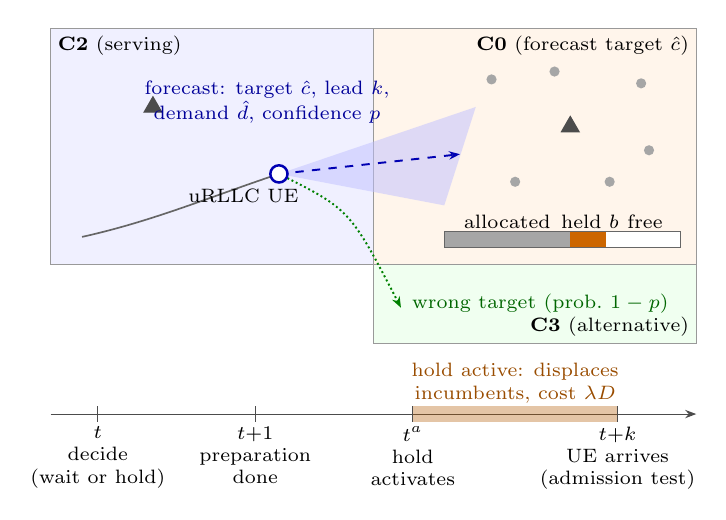
\begin{tikzpicture}[x=1cm,y=1cm,font=\scriptsize,
  tower/.style={draw=black!70,fill=black!70,regular polygon,regular polygon sides=3,inner sep=1.3pt},
  inc/.style={circle,fill=black!35,inner sep=1.3pt},
  lab/.style={align=center,inner sep=1pt}]
  % cells
  \fill[blue!6] (0,0) rectangle (4.1,3.0);
  \fill[orange!8] (4.1,0) rectangle (8.2,3.0);
  \fill[green!6] (4.1,-1.0) rectangle (8.2,0);
  \draw[black!40] (0,0) rectangle (8.2,3.0);
  \draw[black!40] (4.1,-1.0) -- (4.1,3.0);
  \draw[black!40] (4.1,-1.0) -- (8.2,-1.0) -- (8.2,0);
  \node[lab,anchor=north west] at (0.05,2.95) {\textbf{C2} (serving)};
  \node[lab,anchor=north east] at (8.15,2.95) {\textbf{C0} (forecast target $\hat c$)};
  \node[lab,anchor=south east] at (8.15,-0.95) {\textbf{C3} (alternative)};
  % towers
  \node[tower] at (1.3,2.0) {};
  \node[tower] at (6.6,1.75) {};
  % incumbents in C0
  \foreach \p in {(5.6,2.35),(7.5,2.3),(7.6,1.45),(5.9,1.05),(7.1,1.05),(6.4,2.45)} \node[inc] at \p {};
  % RB bar at C0
  \begin{scope}[shift={(5.0,0.22)}]
    \fill[black!35] (0,0) rectangle (1.6,0.2);
    \fill[orange!80!black] (1.6,0) rectangle (2.05,0.2);
    \fill[white] (2.05,0) rectangle (3.0,0.2);
    \draw[black!60] (0,0) rectangle (3.0,0.2);
    \node[lab,anchor=south] at (0.8,0.2) {allocated};
    \node[lab,anchor=south] at (1.85,0.2) {held $b$};
    \node[lab,anchor=south] at (2.55,0.2) {free};
  \end{scope}
  % past path, forecast cone, forecast and alternative paths
  \draw[black!60,line width=0.6pt] (0.4,0.35) .. controls (1.3,0.55) and (2.0,0.85) .. (2.9,1.15);
  \fill[blue!25,opacity=0.5] (2.9,1.15) -- (5.4,2.0) -- (5.0,0.75) -- cycle;
  \draw[blue!70!black,dashed,-{Stealth[length=4pt]},line width=0.7pt] (2.9,1.15) -- (5.2,1.4);
  \draw[green!50!black,densely dotted,-{Stealth[length=4pt]},line width=0.7pt] (2.9,1.15) .. controls (3.8,0.7) .. (4.45,-0.55);
  \node[circle,draw=blue!70!black,fill=white,line width=0.9pt,inner sep=2.2pt] at (2.9,1.15) {};
  \node[lab,anchor=north] at (2.45,1.0) {uRLLC UE};
  \node[lab,anchor=south,text=blue!60!black] at (2.75,1.75) {forecast: target $\hat c$, lead $k$,\\demand $\hat d$, confidence $p$};
  \node[lab,anchor=west,text=green!40!black] at (4.55,-0.5) {wrong target (prob.\ $1-p$)};
  % timeline
  \begin{scope}[shift={(0,-1.9)}]
    \draw[-{Stealth[length=4pt]},black!70] (0,0) -- (8.2,0);
    \fill[orange!70!black,opacity=0.35] (4.6,-0.1) rectangle (7.2,0.1);
    \node[lab,anchor=south,text=orange!60!black] at (5.9,0.1) {hold active: displaces\\incumbents, cost $\lambda D$};
    \foreach \x/\t/\d in {0.6/$t$/decide\\(wait or hold),2.6/$t{+}1$/preparation\\done,4.6/$t^{a}$/hold\\activates,7.2/$t{+}k$/UE arrives\\(admission test)}
      {\draw[black!70] (\x,-0.1) -- (\x,0.1);
       \node[lab,anchor=north] at (\x,-0.12) {\t\\\d};}
  \end{scope}
\end{tikzpicture}
\caption{Problem scenario. A uRLLC UE in C2 is forecast to enter C0 after $k$ intervals with demand $\hat d$ and target confidence $p$. The controller may hold $b$ RBs at C0. The hold protects admission if the forecast is right and C0 is short of capacity, but while active it can displace C0's incumbents, and it is wasted if the UE turns into C3 instead.}
\label{fig:scenario}
\end{figure}

The operator therefore faces a per-UE, per-interval choice: hold now, or wait for a sharper forecast; if holding, decide how much and when the hold should start. The rest of the paper formalizes this choice and learns it.

% ======================================================================
\section{System Model}\label{sec:model}
\subsection{Network, traffic and mobility}
Time advances in intervals of $\Delta t=100$\,ms. $N=32$ UEs move in a $100\times100$ square with four sites at $(25,25)$, $(75,25)$, $(25,75)$ and $(75,75)$. Each cell has $C=60$ RBs. Velocities follow a Gaussian random walk ($\sigma=0.1$ per interval, speed capped at 4 units per interval) with reflecting walls. Each UE belongs to one slice $s$ for the whole run. Its per-interval demand $d$ is a rounded Gaussian (at least one RB) with the slice deviation $\sigma_s$. The mean is the slice mean modulated by a common $\pm16\%$ load cycle with a period of 47 intervals. A uRLLC burst, with probability $0.08$ per interval, multiplies the mean by $1.55$. Table~\ref{tab:slices} lists the slice profiles. A UE is served by its nearest site, and a cell change occurs when the nearest site changes.

\begin{table}[!t]
\centering
\caption{Slice profiles. The admission floor is capped by the UE's demand.}
\label{tab:slices}
\begin{tabular}{lrrrrr}
\toprule
Slice & Mean $d$ & $\sigma_s$ & Floor $f_s$ & Latency & Priority\\
\midrule
eMBB & 10.5 & 3.0 & 7 & 20\,ms & 2\\
uRLLC & 7.0 & 2.0 & 5 & 5\,ms & 3\\
mMTC & 3.2 & 1.2 & 2 & 100\,ms & 1\\
\bottomrule
\end{tabular}
\end{table}

\subsection{Scheduling, admission and outage}
In each interval, every cell serves its connected incumbents in strict slice priority order (uRLLC, eMBB, mMTC; ties broken by UE identifier). The budget is the capacity minus the active holds. A hold therefore displaces incumbent service exactly when the cell has unmet incumbent demand $u_c$. The displacement charged to the holds at cell $c$ is $\min(h_c,u_c)$ RB-intervals, where $h_c$ is the total active hold, apportioned in proportion to each hold's size.

A handover of a UE with demand $d$ and slice floor $f=\min(f_s,d)$ into cell $c$ can use its own active holds at $c$ ($m$ RBs) plus the cell's free RBs $F_c$. It is \emph{admitted} if
\begin{equation}\label{eq:admit}
\min(d,\,m+F_c)\ge f
\end{equation}
is within the slice-specific latency limit, where
$\ell_s\in\{8,2,22\}$\,ms denotes the base latency
of (eMBB, uRLLC, mMTC), respectively.
The cell-load variable $\rho_c$ denotes the load
quantity computed by the simulator at the handover
interval. Its precise normalization and whether
active holds are included must be consistent with
the simulator's load calculation.

The allocation term
$\min(d,m+F_c)/d$ represents the fraction of the
arriving UE's demand that can be served using its
own active reservation and the target cell's
remaining free capacity. The QoS indicator therefore
evaluates the full-demand condition together with
the modeled latency constraint.

\subsection{Reservation contracts}
A hold, or \emph{contract}, specifies a UE, a
target cell, a reservation amount and an intended
activation interval. A request requires
$\delta_p=1$ interval of preparation before
activation. Pending contracts consume no active
resource blocks, but they are included in the
request-time reservation limit.

Let $t_j^a(t')$ denote the scheduled activation
time of a pending contract $j$ at a later interval
$t'$. When a new forecast for the same target cell
becomes available, the contract manager updates
the scheduled activation time according to the
selected timing mode and the updated forecast.
The target cell and reservation amount remain
fixed after contract creation.

An activation is permitted only when the
reservation can be accommodated without
violating the admission floors of the connected
incumbents at the target cell. Otherwise, the
activation is rejected. A contract terminates
when its UE arrives at the target, when it expires
at the forecast horizon, or when it is censored
at the end of the simulation.

\subsection{Forecasting}
A two-hidden-layer perceptron (35--64--32--24, tanh) forecasts each UE's next eight positions and demands from six frames of history. It predicts residuals over a constant-velocity projection. It is trained on \ForecastTrainExamples{} examples from seeds disjoint from validation and test, and reaches a validation position RMSE of \ForecastPosRMSE{} world units and a demand MAE of \ForecastDemandMAE{} RB. Applying the cell-selection rule along the forecast path gives the forecast target cell $\hat c$ and lead $k\in\{1,\dots,8\}$ intervals. The forecaster also reports a single score of \ForecastScore{}, which is the same for every forecast and is not a calibrated probability.

% ======================================================================
\section{Mathematical Formulation}\label{sec:formulation}
\subsection{Decision variables}
A \emph{decision point} $(i,t)$ is a connected UE $i$ with no open contract whose forecast at interval $t$ predicts a change to a cell $\hat c_{i,t}\neq c_i(t)$ at lead $k_{i,t}$. With forecast demand $\hat d_{i,t}$, the controller chooses
\begin{equation}\label{eq:decision}
x_{i,t}\in\{\textsc{wait}\}\cup\big(\mathcal{B}_{i,t}\times\mathcal{T}_{i,t}\big),
\end{equation}
with candidate amounts and activation delays
\begin{align}
\mathcal{B}_{i,t}&=\{\hat f_{i,t},\ \hat d_{i,t},\ \hat d^{+}_{i,t}\},\quad \hat f_{i,t}=\min(f_{s(i)},\hat d_{i,t}),\label{eq:amounts}\\
\hat d^{+}_{i,t}&=\big\lceil \hat d_{i,t}+\sigma_{s(i)}\big\rceil,\qquad
\mathcal{T}_{i,t}=\{0,\ \lfloor k_{i,t}/2\rfloor,\ k_{i,t}-1\}.\label{eq:timing}
\end{align}
A hold $x=(b,\delta)$ creates contract $j$ for UE $i$ at target $\hat c_{i,t}$ with amount $b_j=b$, activation time $t^{a}_j=t+\max(\delta,\delta_p)$ and expiry $t^{e}_j=t+8$. These three timings (\emph{now}, \emph{mid}, \emph{jit}) together with the three amounts give nine hold actions.

\subsection{Objective}
Here, $d_j$ denotes the arrival demand,
$(1+T_o)d_j$ is an analytical one-step valuation
of the service associated with a rescued admission,
$q=4$ RB is the QoS-rescue weight, and
$w_s=(1,2,0.5)$ for (eMBB, uRLLC, mMTC).

The displacement quantity $D_j$ is allocated
proportionally among the active contracts at the
target cell. If $b_j$ is the size of contract $j$,
$h_c$ is the total active reservation at cell $c$,
and $u_c$ is the unmet incumbent demand, its
allocated displacement is

\begin{equation}
D_j =
\begin{cases}
\displaystyle
\frac{b_j}{h_c}\min(h_c,u_c),
& h_c>0,\\[6pt]
0,&h_c=0.
\end{cases}
\label{eq:displacement-allocation}
\end{equation}

This proportional allocation is a budget-balanced
cost-sharing rule across concurrent active holds.
It is not a leave-one-contract-out marginal
counterfactual. The aggregate displacement across
all active contracts equals the additional incumbent
service that would be available if all active holds
were removed simultaneously.

The price $\lambda$ is uniform per displaced RB
and does not weight displacement according to
the slice priority of the affected incumbent.
Consequently, the reward represents an operator-
specified aggregate displacement cost rather than
a slice-weighted measure of incumbent utility.

The term $(1+T_o)d_j$ is a one-step analytical
surrogate evaluated at the arrival interval. It
does not represent an exact multi-interval
counterfactual rollout of the UE's time-varying
demand during the subsequent outage period.
\subsection{Constraints}
Let $\mathcal{U}_c(t)$ be the connected incumbents of cell $c$, $a_u(t)$ the RBs scheduled to UE $u$, $H_c(t)$ the active holds and $P_c(t)$ the pending holds at $c$. The problem is subject to
\begin{align}
&\textstyle\sum_{u\in\mathcal{U}_c(t)}a_u(t)+H_c(t)\le C, &&\forall c,t,\label{eq:cap}\\
&b_j\le C-H_c(t^{a}_j)-\textstyle\sum_{u\in\mathcal{U}_c(t^{a}_j)}f_u(t^{a}_j), &&\forall j,\label{eq:floor}\\
&b_j\le C-H_c(t)-P_c(t) \ \text{at request}, &&\forall j,\label{eq:nooverbook}\\
&t+\delta_p\le t^{a}_j\le t^{e}_j, &&\forall j,\label{eq:timewin}\\
&\text{at most one open contract per UE}. &&\label{eq:onecontract}
\end{align}
Constraint~\eqref{eq:cap} enforces the
instantaneous capacity limit at every cell and
interval.

Constraint~\eqref{eq:nooverbook} is a
request-time constraint. It is checked when a
new contract is proposed and prevents the total
active and pending reservations from exceeding
the cell capacity. The pending-reservation term
$P_c(t)$ includes all currently pending contracts
targeting cell $c$, irrespective of their scheduled
activation intervals. Illegal actions are excluded
using the request-time action mask.

In contrast, Constraint~\eqref{eq:floor} is an
activation-time feasibility condition. The future
incumbent set, active reservations and admission
floors are evaluated when the contract is scheduled
to activate. Since these quantities may change
after the original request, this condition is
enforced by the contract manager as an environment
transition rule. If the required capacity is
unavailable, the activation is rejected.

Constraint~\eqref{eq:timewin} defines the
permitted activation window, while
Constraint~\eqref{eq:onecontract} prevents a UE
from maintaining multiple open contracts
simultaneously.

\subsection{Sequential decision process and optimal stopping}
Problem~\eqref{eq:objective}--\eqref{eq:onecontract}
is a constrained sequential decision problem with
coupled UEs. CARE approximates this problem by
learning per-UE, per-crossing action values.

For each decision point, the policy observes a
state $s$ consisting of 17 causal features
(Section~\ref{sec:care}). The available actions
consist of waiting or committing one of the
candidate reservation contracts.

For a hold action $x$, the immediate value is
the expected contract reward. The waiting action
preserves the option of making a reservation at
a later decision point. Never committing a
contract has a zero continuation value.

The Bellman equations are written as By the Bellman optimality principle~\cite{sutton2018rl}, the optimal action values therefore satisfy
\begin{align}
Q^{*}(s,x)&=\mathbb{E}\left[R_j\mid s,x\right],\qquad x\in\mathcal{B}\times\mathcal{T},\label{eq:qhold}\\
Q^{*}(s,\textsc{wait})&=\gamma\,\mathbb{E}\Big[\max\big(0,\max_{x'}Q^{*}(s',x')\big)\Big],\label{eq:qwait}
\end{align}
where $s'$ is the same UE's next decision state for the same crossing, $\gamma=0.98$, and $Q^{*}(s,\textsc{wait})=0$ if no such state follows. The inner $\max(0,\cdot)$ encodes the option of never holding.

The aggregate displacement allocation in
~\eqref{eq:displacement-allocation} has the
following budget-balance property:
\begin{proposition}\label{prop:displacement}
Under the memoryless priority scheduler, the displacement charged by~\eqref{eq:reward}, summed over all contracts in an interval, equals the extra RBs that incumbents would have received in that interval if every active hold were removed.
\end{proposition}
\begin{IEEEproof}
At cell $c$ with active holds $h_c$, removing the holds raises the scheduling budget by $h_c$. The priority scheduler hands those RBs to unmet incumbents until either the $h_c$ RBs or the unmet demand $u_c$ run out, so incumbents gain $\min(h_c,u_c)$ RBs. The simulator charges exactly this amount, split among the holds at $c$ in proportion to their sizes.
\end{IEEEproof}

% ======================================================================
\section{Proposed Method: CARE}\label{sec:care}
Fig.~\ref{fig:architecture} shows the CARE pipeline. The top row runs in every interval; the bottom row settles contracts, computes counterfactual rewards and, during training, updates the Q-networks.

\begin{figure*}[!t]
\centering
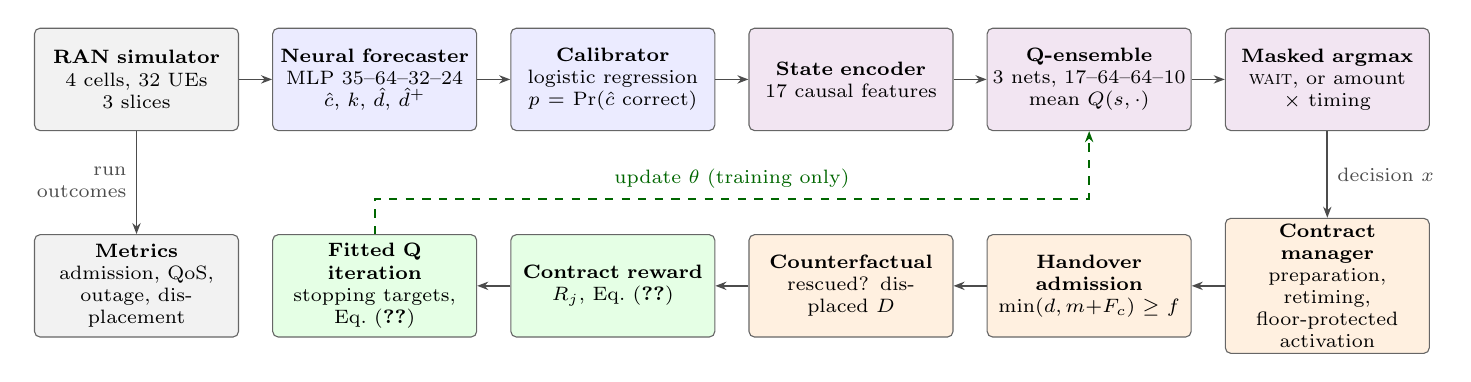
\begin{tikzpicture}[font=\scriptsize,
  box/.style={draw=black!60,rounded corners=2pt,align=center,minimum height=1.3cm,text width=2.45cm,inner sep=2pt},
  pred/.style={box,fill=blue!8},
  dec/.style={box,fill=violet!10},
  con/.style={box,fill=orange!12},
  lrn/.style={box,fill=green!10},
  arr/.style={-{Stealth[length=4pt]},black!70,line width=0.6pt},
  node distance=0.42cm]
  \node[box,fill=black!5] (sim) {\textbf{RAN simulator}\\4 cells, 32 UEs\\3 slices};
  \node[pred,right=of sim] (fc) {\textbf{Neural forecaster}\\MLP 35--64--32--24\\$\hat c$, $k$, $\hat d$, $\hat d^{+}$};
  \node[pred,right=of fc] (cal) {\textbf{Calibrator}\\logistic regression\\$p=\Pr(\hat c$ correct$)$};
  \node[dec,right=of cal] (enc) {\textbf{State encoder}\\17 causal features};
  \node[dec,right=of enc] (q) {\textbf{Q-ensemble}\\3 nets, 17--64--64--10\\mean $Q(s,\cdot)$};
  \node[dec,right=of q] (act) {\textbf{Masked argmax}\\\textsc{wait}, or amount\\$\times$ timing};
  \node[con,below=1.1cm of act] (cm) {\textbf{Contract manager}\\preparation, retiming,\\floor-protected activation};
  \node[con,left=of cm] (adm) {\textbf{Handover admission}\\$\min(d,m{+}F_c)\ge f$};
  \node[con,left=of adm] (cf) {\textbf{Counterfactual}\\rescued? displaced $D$};
  \node[lrn,left=of cf] (rw) {\textbf{Contract reward}\\$R_j$, Eq.~(\ref{eq:reward})};
  \node[lrn,left=of rw] (fqi) {\textbf{Fitted Q iteration}\\stopping targets,\\Eq.~(\ref{eq:targets})};
  \node[box,fill=black!5,left=of fqi] (met) {\textbf{Metrics}\\admission, QoS,\\outage, displacement};
  \draw[arr] (sim) -- (fc);
  \draw[arr] (fc) -- (cal);
  \draw[arr] (cal) -- (enc);
  \draw[arr] (enc) -- (q);
  \draw[arr] (q) -- (act);
  \draw[arr] (act) -- node[right]{decision $x$} (cm);
  \draw[arr] (cm) -- (adm);
  \draw[arr] (adm) -- (cf);
  \draw[arr] (cf) -- (rw);
  \draw[arr] (rw) -- (fqi);
  \draw[arr,dashed,green!40!black] (fqi.north) -- ++(0,0.45) -| node[pos=0.25,above]{update $\theta$ (training only)} (q.south);
  \draw[arr] (sim.south) -- node[left,align=right]{run\\outcomes} (met.north);
\end{tikzpicture}
\caption{CARE pipeline. Blue: prediction. Purple: per-interval decision. Orange: contract mechanics and counterfactual accounting inside the simulator. Green: learning, used only during training. Every policy, rule and ablation in the evaluation shares the same forecaster, calibrator and contract mechanics.}
\label{fig:architecture}
\end{figure*}

\subsection{Calibrated target confidence}
The forecaster returns trajectories, not probabilities. CARE estimates $p=\Pr(\text{next cell change goes to }\hat c)$ by logistic regression on seven observable descriptors: lead, signal margin between target and serving cell, serving signal, speed, heading toward the target, distance gap to the cell bisector, and closing speed. The basis adds two interaction terms (lead $\times$ signal margin, bisector gap $\times$ closing speed), the squared lead and an intercept:
\begin{equation}\label{eq:calibration}
\begin{aligned}
p&=\sigma\!\left(\mathbf{w}^{\top}\phi(\mathbf{z})\right),\\
\mathbf{w}&=\arg\min_{\mathbf{w}}\ \sum_n \mathcal{L}_{\mathrm{log}}\big(y_n,\sigma(\mathbf{w}^{\top}\phi_n)\big)+\tfrac{\kappa}{2}\|\mathbf{w}\|^2,
\end{aligned}
\end{equation}
where $\sigma$ is the logistic function, $y_n=1$ if the forecast target was correct, and $\kappa=10^{-3}$. The model is fit by Newton iterations on \CalFitExamples{} forecasts from 20 dedicated calibration seeds and scored on \CalTestExamples{} forecasts from the 20 test seeds. Observed target accuracy is \CalAccLeadOne\% at a one-interval lead and \CalAccLeadEight\% at eight intervals. A single constant score cannot represent that spread.

\subsection{State and action space}
In every interval, each decision point (up to 32 per interval) is encoded by 17 causal features: calibrated confidence $p$, normalized lead, forecast demand, admission floor, free and floor-protected claimable RBs at the target, the target's incumbent allocation, unmet demand and active holds, the slice one-hot, signal margin, speed, outage length, current demand and a bias. The policy never observes the counterfactual quantities used for credit. The action space~\eqref{eq:decision} has ten actions; actions that would violate~\eqref{eq:nooverbook} are masked.

\subsection{Learning: fitted Q iteration with optimal stopping}
CARE approximates~\eqref{eq:qhold}--\eqref{eq:qwait} with a multilayer perceptron $Q_\theta$ (17--64--64--10, tanh, NumPy) trained by fitted Q iteration~\cite{ernst2005tree,riedmiller2005nfq} on the targets
\begin{equation}\label{eq:targets}
y=\begin{cases}R_j & \text{hold},\\ \gamma\max\big(0,\max_{x'}Q_{\bar\theta}(s',x')\big) & \text{wait, $s'$ exists},\\ 0 & \text{wait, no $s'$},\end{cases}
\end{equation}
where $\bar\theta$ is frozen during each target computation. A committed contract's target is its realized counterfactual reward, which does not depend on the behavior policy, so every transition can be reused. Algorithm~\ref{alg:train} gives the procedure. Data come from an $\epsilon$-greedy behavior policy annealed from uniform over legal actions to $\epsilon=0.05$ over the first 75\% of 240 training episodes of 320 intervals. Every four episodes CARE recomputes the targets twice and fits six epochs of minibatch (512) squared error with Adam~\cite{kingma2015adam} at learning rate $10^{-3}$.

For each price $\lambda\in\{0.25,1,4,16\}$, three replicas are trained from different initializations and trajectory seeds. At run time (Algorithm~\ref{alg:online}), CARE acts greedily on the replicas' \emph{mean} action values. A greedy maximum over nine noisy hold values favors whichever value is overestimated, and averaging independent replicas reduces that variance.

\begin{algorithm}[t]
\caption{CARE training at price $\lambda$ (one replica)}
\label{alg:train}
\begin{algorithmic}[1]
\REQUIRE forecaster, calibrator, price $\lambda$, episodes $E=240$, length $T_{\mathrm{run}}=320$, replica seed $r$
\ENSURE Q-network $Q_\theta$
\STATE initialize $Q_\theta$ with seed $r$; replay buffer $\mathcal{D}\leftarrow\emptyset$
\FOR{$e=0$ \TO $E-1$}
  \STATE $\epsilon\leftarrow$ linear anneal from $1$ to $0.05$ over the first $0.75E$ episodes
  \STATE reset simulator with seed $20000+1000(r-100)+e$
  \FOR{$t=1$ \TO $T_{\mathrm{run}}$}
    \FOR{each decision point $(i,t)$}
      \STATE encode state $s$ with calibrated $p$; legal-action mask $M$
      \STATE $x\leftarrow$ $\epsilon$-greedy over $\{x:M(x)\}$ by $Q_\theta(s,\cdot)$
      \STATE \textbf{if} $x\ne\textsc{wait}$ \textbf{then} create contract $(i,\hat c,b,t^{a})$
    \ENDFOR
    \STATE advance simulator: retime, activate (\ref{eq:floor}), schedule, move, admit (\ref{eq:admit}), settle contracts
  \ENDFOR
  \STATE add $(s,M,x,R_j\text{ or link to next }s')$ of every decision to $\mathcal{D}$
  \IF{$(e+1) \bmod 4=0$}
    \FOR{2 iterations}
      \STATE compute targets $y$ on $\mathcal{D}$ by (\ref{eq:targets}) with frozen $\bar\theta\leftarrow\theta$
      \STATE fit $Q_\theta(s,x)\to y$: 6 epochs, minibatch 512, Adam
    \ENDFOR
  \ENDIF
\ENDFOR
\RETURN $Q_\theta$
\end{algorithmic}
\end{algorithm}

\begin{algorithm}[t]
\caption{CARE online decision in one interval}
\label{alg:online}
\begin{algorithmic}[1]
\REQUIRE trained replicas $Q_{\theta_1},Q_{\theta_2},Q_{\theta_3}$ for the operator's $\lambda$
\FOR{each decision point $(i,t)$}
  \STATE forecast $(\hat c,k,\hat d,\hat d^{+})$; calibrate $p$ by (\ref{eq:calibration})
  \STATE encode $s$ and mask $M$
  \STATE $\bar Q(s,\cdot)\leftarrow\frac13\sum_{m=1}^{3}Q_{\theta_m}(s,\cdot)$
  \STATE $x\leftarrow\arg\max_{x:M(x)}\bar Q(s,x)$
  \STATE \textbf{if} $x\ne\textsc{wait}$ \textbf{then} request hold of $b(x)$ RBs at $\hat c$, activating at $t+\max(\delta(x),\delta_p)$
\ENDFOR
\end{algorithmic}
\end{algorithm}

\subsection{Why not policy gradients}
A natural alternative trains CARE's actor with PPO~\cite{schulman2017ppo} on per-decision Monte Carlo returns, with clip $0.2$ and an entropy bonus annealed from $10^{-2}$ to $10^{-3}$. In that formulation a wait inherits the return of the UE's next \emph{sampled} decision. Because the behavior policy almost always holds at that next decision, waiting and holding receive nearly the same return. There is no gradient toward waiting, and the policy collapses to holding on every forecast, whatever the price. Flooring the sampled continuation at $0$ removes the collapse but overestimates waiting, because a single lucky rescue dominates the sampled maximum. Both PPO variants are reported as ablations (\emph{CARE-PPO w/ on-policy wait} and \emph{CARE-PPO}).

% ======================================================================
\section{Baselines and Experimental Setup}\label{sec:protocol}
\subsection{Simulation settings and seeds}
Table~\ref{tab:params} lists the simulation and training parameters. Seed sets are disjoint by role (Table~\ref{tab:seeds}). Every test run lasts 320 intervals (32\,s) with 32 UEs. All methods on a seed share the mobility, traffic, forecast and radio random streams, so differences between methods are paired. All data are synthetic: they are generated by the simulator from the listed seeds, and no external dataset is used.

\begin{table}[!t]
\centering
\caption{Simulation and training parameters.}
\label{tab:params}
\footnotesize
\setlength{\tabcolsep}{4pt}
\begin{tabular}{ll}
\toprule
Parameter & Value\\
\midrule
Interval $\Delta t$; run length & 100\,ms; 320 intervals\\
Cells; capacity $C$; area & 4; 60 RB each; $100\times100$\\
UEs $N$ & 32 (sweep: 24--48)\\
Mobility & random walk, $\sigma=0.1$, speed $\le4$\\
Load cycle; uRLLC burst & $\pm16\%$, period 47; $p=0.08$, $\times1.55$\\
Radio success; outage $T_o$ & 0.99; 3 intervals\\
Prep.\ delay $\delta_p$; horizon & 1 interval; 8 intervals\\
Forecaster & MLP 35--64--32--24, 6 frames\\
Prices $\lambda$ & 0.25, 1, 4, 16 (main: 1)\\
Reward weights & $w_s=(1,2,0.5)$, $q=4$\\
Q-network & 17--64--64--10, tanh\\
Optimizer & Adam, $10^{-3}$, minibatch 512\\
Discount $\gamma$ & 0.98\\
Episodes; $\epsilon$ & 240; $1\to0.05$ over first 75\%\\
Replicas per $\lambda$ & 3 (seeds 101, 102, 103)\\
PPO (ablation) & 160 episodes, clip 0.2\\
\bottomrule
\end{tabular}
\end{table}

\begin{table}[!t]
\centering
\caption{Seed partitions. No seed is used in more than one role.}
\label{tab:seeds}
\begin{tabular}{ll}
\toprule
Role & Seeds\\
\midrule
Forecaster training / validation & 3000--3023 / 4000--4005\\
Calibration & 4100--4119\\
CARE training (replica $r$) & $20000+1000(r-100)+e$\\
Rule tuning, replica selection & 5000--5009\\
Held-out test & 9000--9019\\
\bottomrule
\end{tabular}
\end{table}

\subsection{Baselines}
All methods use the same forecaster, calibrated confidence and contract mechanics:
\emph{No reservation};
\emph{Reactive} (hold forecast demand immediately, but only once the lead is within the preparation delay plus one interval);
\emph{Certainty-equivalent} (hold forecast demand immediately for every forecast);
\emph{Fixed proactive} (forecast demand at mid-lead when $p\ge0.5$);
\emph{Floor-JIT} (the admission floor, just in time, for every forecast);
\emph{Tuned rule}, the best of 45 (amount, timing, threshold $\tau$) rules on the tuning seeds at each $\lambda$; and
\emph{Slice-tuned rule}, a separately tuned rule per slice, where a slice gets no rule if none has positive utility.

\subsection{Ablations}
\emph{CARE w/o calibration} is trained and run with the forecaster's constant score in place of calibrated confidence. \emph{CARE single network} uses the single replica with the best tuning-seed utility instead of the ensemble. \emph{CARE-PPO} and \emph{CARE-PPO w/ on-policy wait} replace the learner as described in Section~\ref{sec:care} and use the best replica on the tuning seeds. Three mechanism ablations rerun Floor-JIT without retiming, with free (unprotected) activation, and with one decision per interval. A simplified-mechanics run uses unprotected activation, no retiming, no preparation delay and one decision per interval.

\subsection{Metrics and statistics}
We report handover admission rate (HSR), handover QoS rate, outage (share of UE-intervals in re-establishment), whole-network full-service rate, served share of offered RBs, displacement (incumbent RB-intervals displaced, as a share of capacity) and the utility $U_\lambda=J_\lambda$ of~\eqref{eq:objective}, the primary metric. Tables give means over the 20 test seeds with 95\% Student-$t$ half-widths. Comparisons are paired by seed. Two-sided $p$-values come from a sign-flip randomization test (200{,}000 draws), Holm-adjusted~\cite{holm1979simple} over a predeclared family: CARE against each of the seven baselines and four ablations, on $U_1$, HSR, outage and full-service rate (44 tests). Comparisons at the other prices form a second Holm family.

% ======================================================================
\section{Results and Performance Analysis}\label{sec:results}
\subsection{Calibration}
Fig.~\ref{fig:calibration} shows that the calibrated confidence tracks observed target accuracy across its range. The Brier score is \CalBrier{} against \ConstBrier{} for the constant score, the expected calibration error is \CalECE{} against \ConstECE{}, and the AUC is \CalAUC{}. Target accuracy falls from \CalAccLeadOne\% at a one-interval lead to \CalAccLeadEight\% at eight intervals. The base rate is \CalBaseRate\%, so a constant score is right on average but says nothing about \emph{which} forecasts to trust.

\begin{figure}[!t]
\centering
\includegraphics[width=\columnwidth]{calibration.png}
\caption{Left: reliability of calibrated target confidence on the 20 test seeds (bins with at least 20 forecasts). Right: observed target accuracy and mean calibrated confidence by forecast lead.}
\label{fig:calibration}
\end{figure}

\subsection{Main comparison at $\lambda=1$}
Table~\ref{tab:main} and Figs.~\ref{fig:headline} and~\ref{fig:tradeoff} summarize the 20 test seeds. Reservation of any kind matters most. Without it, only \NoResHSR\% of handovers are admitted and UEs spend \NoResOutage\% of UE-intervals in outage. CARE admits \CareHSR\% with \CareOutage\% outage, displacing \CareDisplaced\% of capacity from incumbents. Fig.~\ref{fig:headline} shows that the gain holds for every slice, and that CARE's mean admission is above reactive reservation's in each of them.

\begin{figure*}[!t]
\centering
\includegraphics[width=0.82\textwidth]{headline.png}
\caption{Main result at $\lambda=1$ on the 20 held-out test seeds. Left: handover admission by slice and overall. Right: share of UE-intervals spent in outage after a failed handover. Error bars are 95\% confidence intervals of the mean. CARE and the slice-tuned rule, which use the same calibrated forecasts and floor-protected holds, are close; both clearly improve on no reservation and on reactive reservation.}
\label{fig:headline}
\end{figure*}
 Holding forecast demand for every forecast (Certainty-equivalent) also raises admission, to \CertaintyHSR\%. However, it displaces \CertaintyDisplaced\% of capacity, cuts whole-network full service from \NoResFull\% to \CertaintyFull\%, and its net utility is \CertaintyUtility{} RB per interval: the rescued arrivals are entirely paid for by displaced incumbents.

Against the reactive and fixed baselines, CARE is better on every primary metric. Its utility exceeds Reactive by \VsReactiveUtilDiff{} RB per interval (95\% CI $[\VsReactiveUtilLow,\VsReactiveUtilHigh]$, Holm $p=\VsReactiveUtilP$, 20/20 seeds) and its admission rate by \VsReactiveHSRDiff{} points. Its utility exceeds Fixed proactive by \VsFixedUtilDiff{} ($p=\VsFixedUtilP$).

\textbf{CARE does not outperform the simple rules built on the same ingredients.} Floor-JIT and the two tuned rules reach $U_1$ of \FloorJITUtility{}, \TunedUtility{} and \SliceTunedUtility{}, against \CareUtility{} for CARE. The paired differences are small and negative: \VsFloorJITUtilDiff{} $[\VsFloorJITUtilLow,\VsFloorJITUtilHigh]$, \VsTunedUtilDiff{} $[\VsTunedUtilLow,\VsTunedUtilHigh]$ and \VsSliceTunedUtilDiff{} $[\VsSliceTunedUtilLow,\VsSliceTunedUtilHigh]$. After Holm correction over the 44-test family they are not significant ($p=\VsFloorJITUtilP$, \VsTunedUtilP, \VsSliceTunedUtilP). CARE's whole-network full-service rate is lower by less than a tenth of a point ($\VsSliceTunedFullDiff$ points against the slice-tuned rule, $p=\VsSliceTunedFullP$), and differences in admission and outage are not significant. CARE thus learns a policy whose network outcome is statistically indistinguishable from, and at worst marginally below, a calibrated threshold rule tuned on separate seeds.

All admission-oriented controllers trade QoS for admission. Floor holds admit an arrival at its slice minimum, not its full demand, so CARE's handover QoS rate (\CareQoS\%) is below Reactive's (\ReactiveQoS\%), which holds full demand. Its uRLLC QoS rate is \CareURLLCQoS\% against \ReactiveURLLCQoS\% for Reactive. Utility~\eqref{eq:reward} values a QoS rescue at $q=4$ RB, far less than an admission rescue ($(1+T_o)\,d=42$ RB for a mean eMBB arrival), so every utility-maximizing policy here prefers the floor. An operator who values full-demand handovers more would raise $q$.

\begin{table*}[!t]
\centering
\caption{Held-out results at $\lambda=1$: means over 20 test seeds (32 UEs, 320 intervals). HSR: handover admission rate (\%); QoS: handover QoS rate (\%); Outage: share of UE-intervals in re-establishment (\%); Full: share of UE-intervals receiving full demand, whole network (\%); Served: served share of offered RBs (\%); Displ.: incumbent RB-intervals displaced by holds (\% of capacity); $U_1$: net utility per interval in slice-weighted RBs. Ablations below the line.}
\label{tab:main}
\begin{tabular}{lrrrrrrr}
\toprule
Method & HSR & QoS & Outage & Full & Served & Displ. & $U_{1}$\\
\midrule
No reservation & 51.6 & 45.3 & 5.42 & 75.3 & 79.9 & 0.00 & 0.00\\
Reactive & 83.5 & 66.2 & 1.87 & 74.1 & 80.1 & 1.22 & 10.71\\
Certainty-equivalent & 83.1 & 61.4 & 1.91 & 66.3 & 74.3 & 7.47 & -0.18\\
Fixed proactive & 84.5 & 67.0 & 1.76 & 74.0 & 80.0 & 1.39 & 10.74\\
Floor-JIT & 87.8 & 50.9 & 1.38 & 74.2 & 80.4 & 0.87 & 12.56\\
Tuned rule & 87.8 & 50.9 & 1.38 & 74.2 & 80.4 & 0.85 & 12.59\\
Slice-tuned rule & \textbf{87.9} & 51.0 & 1.37 & 74.3 & 80.4 & 0.84 & 12.65\\
\textbf{CARE (proposed)} & 87.4 & 51.7 & 1.42 & 74.2 & 80.3 & 0.92 & 12.38\\
\midrule
CARE w/o calibration & 84.2 & 52.2 & 1.78 & 74.2 & 80.3 & 0.90 & 12.15\\
CARE single network & 87.5 & 51.8 & 1.41 & 74.1 & 80.3 & 0.99 & 12.40\\
CARE-PPO & 87.8 & 50.9 & 1.38 & 74.2 & 80.4 & 0.87 & 12.56\\
CARE-PPO w/ on-policy wait & 87.8 & 50.9 & 1.38 & 74.2 & 80.4 & 0.87 & 12.56\\
\bottomrule
\end{tabular}
\end{table*}

\begin{figure}[!t]
\centering
\includegraphics[width=\columnwidth]{tradeoff.png}
\caption{Handover admission (left) and whole-network full service (right) against incumbent displacement at $\lambda=1$. Bars are 95\% confidence intervals of the per-method mean. Seed-to-seed variation is large, but all methods are paired by seed.}
\label{fig:tradeoff}
\end{figure}

\subsection{Price response}
The displacement price changes which policy is right. Table~\ref{tab:frontier} and Fig.~\ref{fig:frontier} report utility at each price for the methods that are trained or tuned per price. Floor-JIT has no price parameter and collapses from \LamQuarterFloorJITUtil{} at $\lambda=0.25$ to \LamSixteenFloorJITUtil{} at $\lambda=16$. CARE adapts. The share of its decisions that commit a hold falls from \LamQuarterCareHold\% to \LamSixteenCareHold\%, and its utility stays within $0.6$ RB per interval of the best tuned rule at every price. The gaps (CARE minus tuned rule) are \FrontQuarterTunedDiff{}, \FrontOneTunedDiff{}, \FrontFourTunedDiff{} and \FrontSixteenTunedDiff{} at $\lambda=0.25,1,4,16$.

At $\lambda=16$ the right answer is never to hold, which both tuned rules find. CARE still holds on \LamSixteenCareHold\% of decisions, and its utility differs from theirs by \FrontSixteenTunedDiff{} RB per interval ($p=\FrontSixteenTunedP$, Holm-adjusted within the frontier family). The low-price end shows a different trade. The tuned rule at $\lambda=0.25$ (\TunedRuleQuarter) holds on every forecast and displaces \LamQuarterTunedDisplaced\% of capacity to reach \LamQuarterTunedUtil{}. CARE reaches \LamQuarterCareUtil{} while committing \LamQuarterCareHold\% of decisions and displacing \LamQuarterCareDisplaced\%. When displacement is nearly free, the utility metric rewards the rule. CARE gets within about 4\% of it with about a fifth of the displacement and fewer reservation contracts (\LamQuarterCareContracts{} per run against \LamQuarterTunedContracts{}).

\begin{table}[!t]
\centering
\caption{Held-out utility at each displacement price (RB per interval, 20 seeds) and, in parentheses, the share of forecast decisions that commit a hold. Each method is retrained or retuned for each price; bold is the best mean.}
\label{tab:frontier}
\resizebox{\columnwidth}{!}{\begin{tabular}{lrrrr}
\toprule
Method & $\lambda=0.25$ & $\lambda=1$ & $\lambda=4$ & $\lambda=16$\\
\midrule
Floor-JIT & 14.12 (100\%) & 12.56 (100\%) & 6.30 (100\%) & -18.73 (100\%)\\
Tuned rule & \textbf{14.70 (100\%)} & 12.59 (41\%) & 6.50 (41\%) & \textbf{0.00 (0\%)}\\
Slice-tuned rule & 14.53 (71\%) & \textbf{12.65 (32\%)} & \textbf{6.78 (18\%)} & \textbf{0.00 (0\%)}\\
\textbf{CARE} & 14.10 (24\%) & 12.38 (26\%) & 6.45 (20\%) & -0.25 (2\%)\\
CARE single network & 14.31 (49\%) & 12.40 (65\%) & 5.66 (24\%) & -4.11 (4\%)\\
CARE-PPO & 14.12 (100\%) & 12.56 (100\%) & 0.00 (0\%) & \textbf{0.00 (0\%)}\\
CARE-PPO w/ on-policy wait & -- & 12.56 (100\%) & -- & -18.73 (100\%)\\
\bottomrule
\end{tabular}}
\end{table}

\begin{figure}[!t]
\centering
\includegraphics[width=0.92\columnwidth]{frontier.png}
\caption{Held-out net utility against the displacement price (95\% CIs). The PPO-trained variants collapse either to holding on every forecast or to never holding.}
\label{fig:frontier}
\end{figure}

\subsection{Ablations}
\textbf{Calibration.} Compared with the same learner trained and run on the constant score, CARE admits \nosign{\VsCareUncalHSRDiff} points more handovers ($[\VsCareUncalHSRLow,\VsCareUncalHSRHigh]$, $p=\VsCareUncalHSRP$, \VsCareUncalHSRWins/20 seeds). Its outage changes by \VsCareUncalOutageDiff{} points ($p=\VsCareUncalOutageP$) and its utility by \VsCareUncalUtilDiff{} ($p=\VsCareUncalUtilP$). This is the largest admission effect of any CARE ablation.

\textbf{Learner.} The PPO-trained actors behave as diagnosed in Section~\ref{sec:care} (Fig.~\ref{fig:training}). With the on-policy wait backup, the actor commits a hold on every forecast at every price. On the test seeds it is identical to Floor-JIT, and at $\lambda=16$ CARE's utility exceeds it by \FrontSixteenCarePPOOnPolicyDiff{} RB per interval. With the floored backup, the actor holds on every forecast for $\lambda\le1$ and never for $\lambda\ge4$. At $\lambda=4$, where selective holding pays, CARE's utility exceeds it by \FrontFourCarePPODiff{} RB per interval ($p=\FrontFourCarePPOP$).

\textbf{Ensemble.} The ensemble's utility minus that of the best single replica is \FrontOneCareSingleDiff{} at $\lambda=1$, where holding is rarely costly, and is not significant. It is \FrontFourCareSingleDiff{} at $\lambda=4$ ($p=\FrontFourCareSingleP$) and \FrontSixteenCareSingleDiff{} at $\lambda=16$ ($p=\FrontSixteenCareSingleP$), where a single network's overestimated hold values commit costly holds.

\textbf{Contract mechanics} (Floor-JIT, $\lambda=1$). Removing retiming of pending holds lowers admission from \AblFullHSR\% to \AblNoRetimeHSR\%. With unprotected activation, \AblFreeActReject\% of activations are rejected and admission falls to \AblFreeActHSR\%: the floor-protection rule claims the safe capacity instead of racing incumbents for it. One decision per interval gives \AblSingleHSR\%. Under the simplified mechanics as a whole, proactive reservation lifts admission only from \LegacyNoResHSR\% to \LegacyFixedHSR\%.

\begin{figure}[!t]
\centering
\includegraphics[width=\columnwidth]{training.png}
\caption{Share of training decisions that commit a hold, per price (replica 101, 8-episode moving average). CARE's curves include $\epsilon$-greedy exploration. The PPO actor converges to all-or-nothing policies.}
\label{fig:training}
\end{figure}

\subsection{What CARE learned}
CARE mostly waits (Fig.~\ref{fig:policy}): it waits on \CareWaitURLLC\% of uRLLC, \CareWaitEMBB\% of eMBB and \CareWaitMMTC\% of mMTC decisions. When it commits, it nearly always holds the admission floor (\CareFloorURLLC\%, \CareFloorEMBB\% and \CareFloorMMTC\% of decisions). Forecast-demand and upper-quantile holds are rare (at most \CareDemandURLLC\% and \CareUpperURLLC\%, both for uRLLC). This agrees with the tuned rules, which also chose floor holds (\TunedRule{} at $\lambda=1$). CARE's mean commitment lead is \CareLead{} intervals before arrival, against \FloorJITLead{} for Floor-JIT.

\begin{figure}[!t]
\centering
\includegraphics[width=0.9\columnwidth]{policy.png}
\caption{CARE's decisions by slice at $\lambda=1$ on the test seeds (amount/activation timing).}
\label{fig:policy}
\end{figure}

\subsection{Sensitivity without retraining}
Fig.~\ref{fig:sweeps} varies one condition at a time and keeps every trained and tuned parameter fixed. CARE tracks Floor-JIT and the tuned rule as the re-establishment outage varies (0 to 6 intervals) and as load varies (24 to 48 UEs). At 48 UEs, admission falls to about 53\% for all three, against \SwUesFortyEightNoResHSR\% without reservation. CARE generalizes worse than the rules to a longer preparation delay than it was trained with. At three intervals its admission is \SwPrepThreeCareHSR\% against \SwPrepThreeTunedHSR\% for the tuned rule, because its learned timing assumes that holds activate one interval after the request.

\begin{figure*}[!t]
\centering
\includegraphics[width=0.78\textwidth]{sweeps.png}
\caption{Handover admission when one condition changes and nothing is retrained or retuned (95\% CIs over 20 test seeds).}
\label{fig:sweeps}
\end{figure*}

\subsection{Interactive demonstration}
An interactive web lab replays any seed with CARE and with no reservation side by side, on identical mobility, traffic and radio draws. It shows each decision's calibrated confidence and the ensemble's action values, and it includes the benchmark setting of this paper (test seed 9000).

% ======================================================================
\section{Discussion and Limitations}\label{sec:discussion}
\textbf{What the evidence supports.} Calibrated target confidence and per-contract counterfactual accounting are what make proactive reservation efficient in this model. Removing calibration costs the most admission, and pricing displacement explicitly is what separates the price-aware policies from Floor-JIT. A learned controller trained on these signals reaches the performance of a carefully tuned threshold rule and adapts to the displacement price. It does not surpass the rule, and we do not claim that it does. The negative result about policy gradients is useful on its own: a per-decision credit design that looks natural collapses silently into the trivial policy.

\textbf{Why a rule is hard to beat here.} The decision is close to one-dimensional. Given calibrated confidence and floor-protected just-in-time activation, whether to hold depends mostly on how likely the forecast is to be right, and a threshold captures that. A learned policy has more to offer when the state carries information a rule ignores, such as correlated arrivals, multi-cell congestion and heterogeneous outage costs. With 240 training episodes, CARE's value estimates also remain noisy enough that a rule tuned on 10 seeds is competitive.

\textbf{Future work: choosing the target cell.} CARE reserves at the nearest-site target and never considers sending a UE to a farther but less loaded cell. The simulator already contains a QoS-aware selection rule that scores candidate cells by available capacity, signal, modeled latency and slice floor, with hysteresis and time-to-trigger, but CARE was not evaluated with it. Making the target part of CARE's action would turn reservation into a joint steering-and-holding decision. That multi-cell trade-off cannot be expressed by a single confidence threshold, and it is where a learned controller is most likely to beat a rule. It requires calibrating load-dependent targets and extending the counterfactual to both cells involved.

\textbf{Deployment.} CARE needs only per-UE forecasts, cell loads and the ability to request handover resources. This matches the data-driven closed-loop control that O-RAN exposes through its RAN Intelligent Controllers~\cite{polese2023oran}, so a natural deployment is as a control application at that layer, with the calibrator and Q-ensemble retrained from logged traffic.

\textbf{Limitations.} The simulator abstracts radio, signaling and scheduling. Admission is a capacity check plus a 1\% radio failure, latency is a load-dependent proxy, and the counterfactual is exact only for the memoryless priority scheduler. The topology has four cells and 32 UEs with random-walk mobility. The utility weights ($w_s$, $q$, $T_o$) are modeling choices that change which policy is best. None of these results establish field performance or 3GPP conformance.

\textbf{Reproducibility.} Source code, trained models, raw per-seed results and the scripts behind every table and figure are released with this paper. One command reruns the full pipeline (calibration, training, tuning, held-out evaluation and reporting), and a second regenerates every table, figure and number in this paper from the saved per-seed runs. An automated test checks that the manuscript contains no hand-typed results.

% ======================================================================
\section{Conclusion}\label{sec:conclusion}
CARE treats handover reservation as priced optimal stopping. It uses a calibrated estimate of where a UE is going, credits each hold only for admissions it actually rescues, charges it exactly for the capacity it takes from incumbents, and learns by fitted Q iteration with a Q-ensemble whether, when and how much to hold. On held-out matched seeds, CARE raises handover admission from \NoResHSR\% to \CareHSR\% and adapts its holding to the price of displacement, staying within $0.6$ RB per interval of the best tuned rule at every price. The same evaluation shows that a calibrated threshold rule using the same mechanics is as good or slightly better. For practitioners, the components worth adopting are calibrated confidence, explicit displacement pricing and floor-protected just-in-time holds. Letting the controller choose the target cell is the most promising next step for learning.

% Generated by IEEEtran.bst, version: 1.14 (2015/08/26)
\begin{thebibliography}{10}
\providecommand{\url}[1]{#1}
\csname url@samestyle\endcsname
\providecommand{\newblock}{\relax}
\providecommand{\bibinfo}[2]{#2}
\providecommand{\BIBentrySTDinterwordspacing}{\spaceskip=0pt\relax}
\providecommand{\BIBentryALTinterwordstretchfactor}{4}
\providecommand{\BIBentryALTinterwordspacing}{\spaceskip=\fontdimen2\font plus
\BIBentryALTinterwordstretchfactor\fontdimen3\font minus
  \fontdimen4\font\relax}
\providecommand{\BIBforeignlanguage}[2]{{%
\expandafter\ifx\csname l@#1\endcsname\relax
\typeout{** WARNING: IEEEtran.bst: No hyphenation pattern has been}%
\typeout{** loaded for the language `#1'. Using the pattern for}%
\typeout{** the default language instead.}%
\else
\language=\csname l@#1\endcsname
\fi
#2}}
\providecommand{\BIBdecl}{\relax}
\BIBdecl

\bibitem{foukas2017slicing}
X.~Foukas, G.~Patounas, A.~Elmokashfi, and M.~K. Marina, ``Network slicing in
  {5G}: Survey and challenges,'' \emph{IEEE Communications Magazine}, vol.~55,
  no.~5, pp. 94--100, 2017.

\bibitem{afolabi2018slicing}
I.~Afolabi, T.~Taleb, K.~Samdanis, A.~Ksentini, and H.~Flinck, ``Network
  slicing and softwarization: A survey on principles, enabling technologies,
  and solutions,'' \emph{IEEE Communications Surveys \& Tutorials}, vol.~20,
  no.~3, pp. 2429--2453, 2018.

\bibitem{3gpp28541}
{3GPP}, ``Management and orchestration; {5G} network resource model ({NRM});
  stage 2 and stage 3,'' 3GPP TS 28.541, Release 17, 2023.

\bibitem{3gpp38300}
------, ``{NR}; {NR} and {NG-RAN} overall description; stage 2,'' 3GPP TS
  38.300, Release 17, 2023.

\bibitem{hong1986guard}
D.~Hong and S.~S. Rappaport, ``Traffic model and performance analysis for
  cellular mobile radio telephone systems with prioritized and nonprioritized
  handoff procedures,'' \emph{IEEE Transactions on Vehicular Technology},
  vol.~35, no.~3, pp. 77--92, 1986.

\bibitem{levine1997shadow}
D.~A. Levine, I.~F. Akyildiz, and M.~Naghshineh, ``A resource estimation and
  call admission algorithm for wireless multimedia networks using the shadow
  cluster concept,'' \emph{IEEE/ACM Transactions on Networking}, vol.~5, no.~1,
  pp. 1--12, 1997.

\bibitem{choi1998predictive}
S.~Choi and K.~G. Shin, ``Predictive and adaptive bandwidth reservation for
  hand-offs in {QoS}-sensitive cellular networks,'' in \emph{Proceedings of ACM
  SIGCOMM}, 1998, pp. 155--166.

\bibitem{wu2026prens}
B.~Wu, P.~C. Amogh, N.~V. Abhishek, and M.~Gurusamy, ``{PreNS}: A hybrid
  predictive and real-time resource allocation framework for {5G} and beyond
  {RAN} network slicing,'' \emph{IEEE Transactions on Cognitive Communications
  and Networking}, vol.~12, pp. 7416--7429, 2026.

\bibitem{li2020mobility}
R.~Li, C.~Wang, Z.~Zhao, R.~Guo, and H.~Zhang, ``The {LSTM}-based advantage
  actor-critic learning for resource management in network slicing with user
  mobility,'' \emph{IEEE Communications Letters}, vol.~24, no.~9, pp.
  2005--2009, 2020.

\bibitem{bega2020deepcog}
D.~Bega, M.~Gramaglia, M.~Fiore, A.~Banchs, and X.~Costa-Perez, ``{DeepCog}:
  Optimizing resource provisioning in network slicing with {AI}-based capacity
  forecasting,'' \emph{IEEE Journal on Selected Areas in Communications},
  vol.~38, no.~2, pp. 361--376, 2020.

\bibitem{gharehgoli2023uncertainty}
A.~Gharehgoli, A.~Nouruzi, N.~Mokari, P.~Azmi, M.~R. Javan, and E.~A.
  Jorswieck, ``{AI}-based resource allocation in end-to-end network slicing
  under demand and {CSI} uncertainties,'' \emph{IEEE Transactions on Network
  and Service Management}, vol.~20, no.~3, pp. 3630--3651, 2023.

\bibitem{phyu2023mlslicing}
H.~P. Phyu, D.~Naboulsi, and R.~Stanica, ``Machine learning in network
  slicing---a survey,'' \emph{IEEE Access}, vol.~11, pp. 39\,123--39\,153,
  2023.

\bibitem{park2024proactive}
H.-S. Park, H.~Kim, C.~Lee, and H.~Lee, ``Mobility management paradigm shift:
  From reactive to proactive handover using {AI/ML},'' \emph{IEEE Network},
  vol.~38, no.~2, pp. 18--25, 2024.

\bibitem{manalastas2023hofailure}
M.~Manalastas, M.~U. Bin~Farooq, S.~M.~A. Zaidi, A.~Ijaz, W.~Raza, and
  A.~Imran, ``Machine learning-based handover failure prediction model for
  handover success rate improvement in {5G},'' in \emph{Proceedings of the IEEE
  20th Consumer Communications \& Networking Conference (CCNC)}, 2023, pp.
  684--685.

\bibitem{azimi2022drlslicing}
Y.~Azimi, S.~Yousefi, H.~Kalbkhani, and T.~Kunz, ``Energy-efficient deep
  reinforcement learning assisted resource allocation for {5G-RAN} slicing,''
  \emph{IEEE Transactions on Vehicular Technology}, vol.~71, no.~1, pp.
  856--871, 2022.

\bibitem{villota2022admission}
W.~F. Villota-Jacome, O.~M.~C. Rendon, and N.~L.~S. da~Fonseca, ``Admission
  control for {5G} core network slicing based on deep reinforcement learning,''
  \emph{IEEE Systems Journal}, vol.~16, no.~3, pp. 4686--4697, 2022.

\bibitem{platt1999probabilistic}
J.~C. Platt, ``Probabilistic outputs for support vector machines and
  comparisons to regularized likelihood methods,'' in \emph{Advances in Large
  Margin Classifiers}, A.~J. Smola, P.~Bartlett, B.~Sch{\"o}lkopf, and
  D.~Schuurmans, Eds.\hskip 1em plus 0.5em minus 0.4em\relax Cambridge, MA: MIT
  Press, 2000, pp. 61--74.

\bibitem{guo2017calibration}
C.~Guo, G.~Pleiss, Y.~Sun, and K.~Q. Weinberger, ``On calibration of modern
  neural networks,'' in \emph{Proceedings of the 34th International Conference
  on Machine Learning}, ser. PMLR, vol.~70, 2017, pp. 1321--1330.

\bibitem{brier1950verification}
G.~W. Brier, ``Verification of forecasts expressed in terms of probability,''
  \emph{Monthly Weather Review}, vol.~78, no.~1, pp. 1--3, 1950.

\bibitem{cohen2023conformal}
K.~M. Cohen, S.~Park, O.~Simeone, and S.~Shamai~(Shitz), ``Calibrating {AI}
  models for wireless communications via conformal prediction,'' \emph{IEEE
  Transactions on Machine Learning in Communications and Networking}, vol.~1,
  pp. 296--312, 2023.

\bibitem{foerster2018coma}
J.~N. Foerster, G.~Farquhar, T.~Afouras, N.~Nardelli, and S.~Whiteson,
  ``Counterfactual multi-agent policy gradients,'' in \emph{Proceedings of the
  AAAI Conference on Artificial Intelligence}, vol.~32, no.~1, 2018, pp.
  2974--2982.

\bibitem{ernst2005tree}
D.~Ernst, P.~Geurts, and L.~Wehenkel, ``Tree-based batch mode reinforcement
  learning,'' \emph{Journal of Machine Learning Research}, vol.~6, pp.
  503--556, 2005.

\bibitem{riedmiller2005nfq}
M.~Riedmiller, ``Neural fitted {Q} iteration -- first experiences with a data
  efficient neural reinforcement learning method,'' in \emph{Machine Learning:
  ECML 2005}, ser. Lecture Notes in Computer Science, vol. 3720.\hskip 1em plus
  0.5em minus 0.4em\relax Springer, 2005, pp. 317--328.

\bibitem{eldeeb2025offline}
E.~Eldeeb and H.~Alves, ``Offline and distributional reinforcement learning for
  radio resource management,'' in \emph{Proceedings of the Joint European
  Conference on Networks and Communications \& {6G} Summit (EuCNC/6G Summit)},
  2025, pp. 1--6.

\bibitem{schulman2017ppo}
J.~Schulman, F.~Wolski, P.~Dhariwal, A.~Radford, and O.~Klimov, ``Proximal
  policy optimization algorithms,'' \emph{arXiv preprint arXiv:1707.06347},
  2017.

\bibitem{sutton2018rl}
R.~S. Sutton and A.~G. Barto, \emph{Reinforcement Learning: An Introduction},
  2nd~ed.\hskip 1em plus 0.5em minus 0.4em\relax MIT Press, 2018.

\bibitem{kingma2015adam}
D.~P. Kingma and J.~Ba, ``Adam: A method for stochastic optimization,'' in
  \emph{International Conference on Learning Representations}, 2015.

\bibitem{holm1979simple}
S.~Holm, ``A simple sequentially rejective multiple test procedure,''
  \emph{Scandinavian Journal of Statistics}, vol.~6, no.~2, pp. 65--70, 1979.

\bibitem{polese2023oran}
M.~Polese, L.~Bonati, S.~D'Oro, S.~Basagni, and T.~Melodia, ``Understanding
  {O-RAN}: Architecture, interfaces, algorithms, security, and research
  challenges,'' \emph{IEEE Communications Surveys \& Tutorials}, vol.~25,
  no.~2, pp. 1376--1411, 2023.

\end{thebibliography}

\end{document}
